%%%%%%%%%%%%%%%%%%%%%%%%%%%%%%  IEEEsample.tex
%%%%%%%%%%%%%%%%%%%%%%%%%%%%%%%%%%%%%%%%%
%%%%%%%%%%%%%%%%%%%%%%%    More information: see the header of IEEEtran.sty
%%%%%%%%%%%%%%%%%%%%%%%
%%%%%%%%%%%%%%%%%%%%%%%%%%%%%%%%%%%%%%%%%%%%%%%%%%%%%%%%%%%%%%%%%%%%%%%%%%%%%%%%
%%%%

\documentclass[10pt,twoside]{IEEEtran}
%\documentclass[conference]{IEEEtran}

%%%\IEEEoverridecommandlockouts

\usepackage[ruled]{./algorithm2e}
%%for algorithm2e package, label has to be following caption in the same line!!!
\renewcommand{\algorithmcfname}{ALGORITHM}
\SetAlFnt{\small}
\SetAlCapFnt{\small}
\SetAlCapNameFnt{\small}
\SetAlCapHSkip{0pt}
\IncMargin{-\parindent}

%% \RequirePackage{times}
%% \RequirePackage{algorithmic}
%% \PassOptionsToPackage{boxed}{algorithm}
%% \RequirePackage{algorithm}
%% \RequirePackage{multicol}
%\renewcommand{\algorithmicrequire}{\textbf{Inputs:}}
%\renewcommand{\algorithmicensure}{\textbf{Outputs:}}
%\DeclareMathAlphabet{\mathtsl}{OT1}{ptm}{m}{sl}

%\def\BibTeX{{\rm B\kern-.05em{\sc i\kern-.025em b}\kern-.08em1
%    T\kern-.1667em\lower.7ex\hbox{E}\kern-.125emX}}

%\newtheorem{theorem}{Theorem}
%\newtheorem{lemma}{Lemma}
%\newtheorem{example}{Example}
%\newtheorem{corollary}{Corollary}

\RequirePackage{amssymb, mathptm}
\usepackage{amsbsy}
\usepackage{graphicx}
\usepackage{helvet}
\usepackage{enumerate}
\usepackage{amsmath}
\usepackage{amsfonts}
\usepackage{graphicx}
\usepackage{multirow}
\usepackage{subfig}
\usepackage{comment}



%%indent in algorithm


%\setcounter{page}{1}


% New command for the table notes.
\def\tabnote#1{{\small{#1}}}

% New command for the line spacing.
\newcommand{\ls}[1]
    {\dimen0=\fontdimen6\the\font
     \lineskip=#1\dimen0
     \advance\lineskip.5\fontdimen5\the\font
     \advance\lineskip-\dimen0
     \lineskiplimit=.9\lineskip
     \baselineskip=\lineskip
     \advance\baselineskip\dimen0
     \normallineskip\lineskip
     \normallineskiplimit\lineskiplimit
     \normalbaselineskip\baselineskip
     \ignorespaces
    }
%\renewcommand{\algorithmicrequire}{\textbf{Input:}}
%\renewcommand{\algorithmicensure}{\textbf{Output:}}

\newcommand{\beq}{\begin{equation}}
\newcommand{\eeq}{\end{equation}}
\newcommand{\beqarr}{\begin{eqnarray}}
\newcommand{\eeqarr}{\end{eqnarray}}
%\newcommand{\ov}{\overline}
\newcommand{\ov}{\bar}
\newcommand{\xor}{\bigoplus}
\newcommand{\Fm}{{\mathbb{F}}}



%the following is for space before and after align or other equation environment.

%%
\newtheorem{Algorithm}{Algorithm}[section]
\newtheorem{Definition}{Definition}[section]
\newtheorem{Example}{Example}[section]
\newtheorem{Proposition}{Proposition}[section]
\newtheorem{Lemma}{Lemma}[section]
\newtheorem{Theorem}{Theorem}[section]
\newtheorem{Corollary}{Corollary}[section]
\newtheorem{Conjecture}{Conjecture}[section]
\newtheorem{Problem}{Problem}[section]
\newtheorem{Notation}{Notation}[section]
\newtheorem{Setup}{Problem Setup}[section]

%%%

%%set spacing between table columns
\setlength{\tabcolsep}{3pt}

\begin{document}

%\thispagestyle{empty}
%\pagestyle{empty}

%\ls{1.5}

\title{\large{\textsc{Word-Level Abstraction from
      Bit-Level Circuits using Gr\"obner Bases}}}
%\author{Tim Pruss\\
%A Master's Thesis Proposal\\
%Electrical \& Computer Engineering, University of Utah\\
%Spring Semester 2013
%}

\author{

\IEEEauthorblockN{Tim Pruss\IEEEauthorrefmark{1}, Priyank
  Kalla\IEEEauthorrefmark{1}, Florian Enescu\IEEEauthorrefmark{2}\\}
%\thanks{This work is sponsored in part by a grant from NSF \#CCF-546859.}
\IEEEauthorblockA{\IEEEauthorrefmark{1}Electrical \& Computer
  Engineering, University of Utah\\
\IEEEauthorrefmark{2}Mathematics \& Statistics, Georgia State
University \vspace{-0.25in}
 %\{lv, kalla\}@eng.utah.edu
}
%% \and
%% \IEEEauthorblockN{Florian Enescu\\} 
%% %\thanks{\normalsize  978-3-9810801-8-6/DATE12/$\copyright 2012$ EDAA}
%% \IEEEauthorblockA{Mathematics \& Statistics, Georgia State University
%% % fenescu@mathstat.gsu.edu
%% } 
}
 
\maketitle

%\markboth{MS Proposal by Tim Pruss}{}
\newcommand{\Fq}{{\mathbb{F}}_{q}}
\newcommand{\Fkk}{{\mathbb{F}}_{2^k}}
\newcommand{\Fkkx}[1][x]{\ensuremath{\mathbb{F}}_{2^k}[#1]\xspace}
\newcommand{\Grobner}{Gr\"{o}bner\xspace}
\newcommand{\B}{{\mathbb{B}}}
\newcommand{\Z}{{\mathbb{Z}}}
\newcommand{\F}{{\mathcal{F}}}
\newcommand{\G}{{\mathcal{G}}}
%%%

\newcommand{\debug}[1]{\textcolor{gray}{[ #1 ]}}


%\thispagestyle{empty}
%\pagestyle{empty}

%%%%%%%%%%%%%%%%%%%% Include your files here %%%%%%%%%%%%%%%%%%%%%
\begin{abstract}
A combinational circuit with $k$-inputs and $k$-outputs implements 
Boolean functions $f: \B^k \rightarrow \B^k$, where $\B = \{0, 1\}$.
The function can also be construed as a mapping $f: \Fkk
\rightarrow \Fkk$,  where $\Fkk$ denotes a Galois field of $2^k$
elements. Every function over $\Fkk$ is a polynomial function ---
i.e. there exists a unique, minimal, canonical polynomial
$\F$ that describes $f$. This paper presents novel techniques based on 
computer-algebra and algebraic-geometry to derive the canonical
(word-level) polynomial representation of the circuit as $Y = \F (A)$
over $\Fkk$, where $A$ and $Y$ denote, respectively, the input and 
output bit-vectors of the circuit. We show that this can be achieved
by computing a Gr\"obner basis of a set of polynomials derived from
the circuit, using a specific elimination term order. Our approach can
be generalized to circuits with arbitrary number of inputs and
outputs, as polyfunctions $f: \Fkk^d \rightarrow \Fkk$ or $f:
{\mathbb{F}}_{2^n} \rightarrow {\mathbb{F}}_{2^m}$. 

Computing Gr\"obner bases using elimination orders is, however,
practically infeasible for large circuits. To overcome this
limitation, we present improvements to the computation
based on: i) term orders derived from the topological
traversal of the given circuit; and ii) the use of FGLM algorithm from 
algebraic geometry. We apply our approach to ``reverse-engineer''
hardware implementations of Elliptic Curve Cryptography (ECC)
primitives over Galois fields $\Fkk$ --- with applications to design
verification and function identification. 
\end{abstract}

\section{Introduction}

Abstraction of word-level functionality from bit-level descriptions of
digital circuits is an important fundamental problem in Electronic
Design Automation (EDA) and design verification. Word-level abstractions
find applications in high-level/RTL datapath synthesis
%\cite{demicheli:iccad_98} \cite{demicheli:dac_99}
\cite{demicheli:tcad_03}, RTL verification \cite{WLS} %\cite{arditi:bmd}
\cite{lpsat}, word-level SMT and constraint solving \cite{ms:research}
\cite{boolector}, %\cite{tew:iccad08}, 
etc. Functional abstraction can
also be helpful in detecting malicious modifications to a circuit --
potentially inserted as hardware Trojan horses -- by
{\it reverse-engineering} the function implemented by the circuit\footnote{A
hardware Trojan modifies the functionality of the 
circuit. Abstraction of the function at word-level can perhaps give
some insights into the functional {\it intent} of the Trojan. This can
also be helpful in Trojan classification; such efforts are
currently underway within the EDA community \cite{Bhunia:Trojan}.}. 
It is further desirable that the obtained word-level abstraction be a
{\it canonical} representation of the function, to facilitate
equivalence verification between a specification model and an
implementation circuit. 

This paper presents a symbolic method to derive the {\it word-level,
  canonical, polynomial representation} from a given combinational
circuit. Our approach models the problem over Galois fields, and employs
concepts from commutative algebra and algebraic geometry ---
notably, Gr\"obner bases \cite{ideals:book} theory and
technology --- to derive the word-level abstraction.
%Buchberger's algorithm
%\cite{buchberger_thesis}, elimination ideals 
%and the FGLM algorithm \cite{fglm}. 

The main motivation for this work is to ``reverse engineer'' (or
to identify) the function implemented by a given Galois field
arithmetic circuit as used in Elliptic Curve Cryptography (ECC). The
main operations of encryption, decryption and authentication in ECC
rely on point-addition and point-doubling operations on elliptic
curves defined over Galois fields $\Fkk$. These primitive operations
are, in turn, implemented as circuits that perform polynomial
computations over $k$-bit vectors \cite{eccld}. 
%Moreover, the datapath size $k$ in these applications
%can be very large, {\it e.g.} $k = 163, 233$ and larger, as specified
%by the US National Institute for Standards and Technology (NIST) for
%ECC. 
The objective is to apply our approach to a given circuit and
{\it extract  the word-level polynomial function (polyfunction)}
implemented by it for design verification. While our approach can be
applied to any arbitrary combinational circuit, it is most beneficial
for arithmetic circuits where canonical Boolean representations prove
to be infeasible. 


{\bf Problem Statement:} Given a combinational circuit $C$ with
$k$-bit inputs and $k$-bit outputs, such that the circuit implements 
Boolean functions that are mappings between $k$-dimensional Boolean
spaces: $f: \B^k \rightarrow \B^k$. Let $\{a_0, \dots, a_{k-1}\}$
denote the primary inputs of the circuit, and let $\{y_0, \dots,
y_{k-1}\}$ denote the bit-level primary outputs. Suppose that we do
not know the function implemented by the circuit. We wish to
derive a {\it word-level, symbolic representation} of the function as
$Y = \F(A)$ over $\Fkk$, where $Y = \{y_0, \dots, y_{k-1}\}$, $A =
\{a_0, \dots,  a_{k-1}\}$ are, respectively, the output and input
bit-vectors (words), and $\F$ denotes a polynomial representation of
the function $f$. We wish to further generalize our approach to any
circuit with arbitrary number  of inputs ($n$) and outputs ($m$), as
polyfunctions $f: {\mathbb{F}}_{2^n} \rightarrow
{\mathbb{F}}_{2^m}$. 

{\bf Approach:} Canonical symbolic DAG 
representations of Boolean functions, such
as ROBDDs \cite{BRYA86}, FDDs \cite{okfdd}, BMDs \cite{bmd}, etc., are
based on (variants of) the Shannon's  expansion, which is a bit-wise,
Boolean decomposition. These are inapplicable to 
word-level abstraction of modulo-arithmetic circuits over Galois
extension fields $\Fkk$. Therefore, we approach this problem from the
perspective of {\it symbolic computer algebra and algebraic geometry}. 

The function $f: \B^k \rightarrow \B^k$ is a
mapping among $2^k$ elements. Therefore, $f$ can also be interpreted,
algebraically, in the following two ways: i) as a function $f:
\Z_{2^k} \rightarrow \Z_{2^k}$, i.e. as a function over finite integer
rings $\pmod{ 2^k}$; and ii) as a function $f: \Fkk \rightarrow \Fkk$,
where $\Fkk$ represents the Galois field of $2^k$
elements. In this work, we will analyze $f$ as a polynomial function
over $\Fkk$, for the following reasons. 

First of all, {\it not every
  function} of the type $f: \Z_{2^k} \rightarrow \Z_{2^k}$, is a
polynomial function; i.e. every function cannot be represented by a
polynomial $\F \pmod{ 2^k}$.  In commutative algebra, identification of
such polynomial functions is an important problem: given a function
$f: \Z_n \rightarrow \Z_n$, $n \in {\mathbb{N}}$, identify if $f$ has
a polynomial representation. If so, derive a unique,
minimal, canonical polynomial $\F$, such that $f \equiv  \F \pmod{
  n}$. 
%that represents $f$. 
%This
%requires to analyze $f$ at each of the $n$ points, and to setup a
%system of $n$ linear congruences to solve. If this system of
%congruences has a solution, then $f$ is a polynomial function; 
%otherwise, $f$ is not a polynomial function. And the feasible
%solutions to these linear congruences correspond to the coefficients
%of a polynomial $\F$ that represents $f$.  
The work of 
\cite{singmaster} 
%\cite{chen_95} \cite{chen_96} 
addresses such problems in number theory and algebra. {\it
 Shekhar et al.} \cite{shekhar:tcad07} address RTL verification
of polynomial datapaths over $k$-bit vectors using the above
concepts. However, in their work, the RTL datapath is already known to
be a polynomial function $\pmod{ 2^k}$. Unfortunately, an arbitrary
$k$-input/$k$-output combinational circuit cannot always be modeled as
a polynomial function over $\Z_{2^k}$; therefore, the $\Z_{2^k}$ model
is not considered in this work. 

On the other hand, there is a well-known ``textbook'' result
\cite{ff:1997} which states that over Galois fields ($\Fq$) of $q$
elements, {\it every function} $f: \Fq \rightarrow \Fq$ is a
polynomial function. 
%By analyzing $f$ over each of the $q$ points, one can apply
%Langrange's interpolation formula and interpolate a polynomial $\F(x)
%= \sum_{k=1} ^q  \frac{ \prod_{i \neq k}  (x -x_i)}{\prod_{i \neq k}
%  (x_k -x_i)} \cdot f(x_k)$, which is a polynomial of degree at 
%most $q-1$ in $x$. One can easily see that $\F(a)=f(a)$ for all $a \in
%\Fq$, and $\F(x)$ is therefore the polynomial function representation
%of $f$. 
Motivated by this fundamental result, we devise an approach
to derive a word-level polynomial function abstraction from the
circuit using the $f: \Fkk \rightarrow \Fkk$ polyfunction model. 
%Given the circuit $C$ which represents a function $f:
%\B^k \rightarrow \B^k$, we interpret $f$ as a function $f: \Fkk
%\rightarrow \Fkk$, and derive a unique, minimal, canonical polynomial
%representation as $Y = \F(A)$ over $\Fkk$, where $Y, A$ are,
%respectively, the output and input bit-vectors of the circuit
%$C$. 
%Note, however, that we are not given a function (mapping);
%rather, we are given a circuit, which is an encoding of the
%function. Interpolating a polynomial $\F$ over $2^k$ points is
%also going to be infeasible for large values of $k$. Therefore, 
We analyze the circuit, derive a specific set of polynomials modeled
over $\Fkk$, and compute a {\it Gr\"obner basis} of these polynomials
with a specific term order to abstract the canonical polynomial
representation. Our approach can be generalized to a circuit with
arbitrary number of inputs and outputs, i.e. to model polynomial
functions $f: \Fkk^d \rightarrow \Fkk$, and further to $f:
{\mathbb{F}}_{2^n} \rightarrow {\mathbb{F}}_{2^m}$.  


%\subsection{Contributions of this Thesis}
{\bf Approach \& Contributions:} 

\begin{enumerate}
\item Using polynomial abstractions, we analyze the circuit, and
  model the gate-level Boolean operators as elements of a multivariate
  polynomial ring with coefficients in $\Fkk$.

\item Based on the concepts of {\it Strong Nullstellensatz, Gr\"obner
  bases, elimination ideals and projections of varieties}
  \cite{ideals:book}, we deduce that the polynomial abstraction
  problem can be formulated as one of {\it computing a Gr\"obner
    basis} of a set of polynomials derived from the given circuit
  netlist, using a specific elimination term order $>$. 

\item Computing Gr\"obner bases using elimination term orders is
  infeasible for large circuits. To overcome this limitation, we 
  investigate the use of the FGLM algorithm \cite{fglm} to derive the
  polynomial representation. The FGLM algorithm takes an {\it already
    computed} Gr\"obner basis ($G_1$) w.r.t. an arbitrary term order
  $>_1$, and transforms it into another Gr\"obner basis ($G$)
  w.r.t. an elimination term order $>$. In the work of {\it
  Lv} \cite{lv:date2012} it was shown that for any
  given circuit, there exists a term order $>_1$ that renders the set
  of polynomials derived from the circuit itself a Gr\"obner
  basis. Moreover, $>_1$ can be easily derived by performing a reverse
  topological traversal of the circuit. Consequently, $G_1$ is readily
  available as a Gr\"obner basis directly by construction. Using FGLM,
  we can then translate $G_1$ into the Gr\"obner basis $G$
  w.r.t. the required elimination order $>$. 

\item The worst-case complexity of computing a Gr\"obner basis is
  known to be doubly exponential in $n$, the number of variables, and
  polynomial in $d$, the degree of the ideal. Most hardware/software
  verification applications do exhibit such high complexity, as the
  number of intermediate computations in the Gr\"obner basis algorithm
  (Buchbeger's algorithm) \cite{buchberger_thesis} 
  tend to explode. Therefore, we conjecture that using the FGLM
  algorithm --- which relies on {\it sparse linear algebra concepts}
  --- perhaps this complexity can be avoided. We are currently
  implementing a domain specific FGLM algorithm --- specifically for
  the abstraction problems related to Galois field
  crypto-circuits. Experimental results with FGLM are not yet available.

%\item As an application, we will use our CAD approach to
%  reverse-engineer the function implemented by a given Galois field
%  arithmetic circuits used in ECC   implementations. This can be used
%  for function identification from a given circuit for formal
%  verification. 

\end{enumerate}

{\bf Paper Organization:} The next section reviews previous work in
the area of canonical representations functions, word-level
abstractions, 
%formal design verification using computer algebra techniques, 
and also polynomial interpolation literature in symbolic
computing. Section \ref{sec:prelimgf} reviews 
Galois field theory and describes the arithmetic circuits that we wish
to verify using our approach. Section \ref{sec:ideals}
reviews preliminary computer-algebra concepts related to ideals,
varieties, Gr\"obner bases, elimination ideals and
Nullstellensatz. Section \ref{sec:theory} describes our results on
polynomial abstraction from circuits, and demonstrates the application
of our work using preliminary experiments. The application of the FGLM
algorithm is covered in Section \ref{sec:fglm}. Finally, Section
\ref{sec:concl} concludes the proposal. 

\section{Review of Previous Work}
\label{sec:prev}

{\bf Canonical Decision Diagrams:} 
The Reduced Ordered Binary Decision Diagram
(ROBBD) \cite{BRYA86}, based on the Shannon's decomposition, was the
first significant contribution in this area. 
Motivated by the success of BDDs, 
variants of the Shannon's decomposition principle (Davio,
Reed-Muller, etc.) were explored to develop other functional decision
diagrams: FDDs \cite{okfdd}, ADDs \cite{add}, %MTBDDs\cite{mtbdd},  
HDDs \cite{hdd} and EVBDDs \cite{evbdd}. 
%While these are %{\it curiously} still 
%referred to as {\it Word-Level Decision Diagrams} \cite{WLS}, 
Binary Moment Diagrams (BMDs) \cite{bmd}, and its derivative K*BMDs
\cite{kbmd}, % and *PHDDs \cite{phdd}, 
depart from the Boolean
decomposition and perform the decomposition of a {\it linear} function
based on its two moments. The decomposition is still point-wise,
binary, w.r.t. each Boolean variable; these do not
serve the purpose of word-level abstraction from bit-level
representations. 

%% BMDs provide a compact representation for
%% integer arithmetic circuits such as multipliers and squarers. However,
%% these are inapplicable for modulo-arithmetic circuits over Galois fields.
%in our application, we encounter modulo-arithmetic circuits and that
%too over Galois fields. For such applications, these representations
%are inapplicable. Taylor Expansion Diagrams (TEDs) \cite{ted_tcomp}
%generalize the linear moment decomposition of BMDs into a Taylor
%series expansion --- this allows the representation of RTL
%descriptions as polynomials over bit-vectors. However, 
Taylor Expansion Diagrams (TEDs) \cite{ted_tcomp} are a word-level
canonical representation of a {\it polynomial expression}, but they do
not represent a {\it polynomial function} canonically. 
%For example, $f_1 = 0$ and $f_2 = 2x^2 - 2x
%\pmod{ 4}$ are two different polynomial representations of the zero
%function over $\Z_4$; but they are symbolically different
%polynomials and they have different (non-isomorphic) TED DAGs. 
While \cite{shekhar:tcad07}  and \cite{alizadeh:tcad2010} provide
canonical representations of polynomial functions, they do so over
$\Z_{2^k}$ and not over $\Fkk$.
%finite integer rings and not over Galois fields.  


MODDs \cite{modd} \cite{modd_tcomp} are a DAG representation of the
characteristic function of a circuit over Galois fields $\Fkk$. MODDs
come very close to satisfying our requirements as a canonical
word-level representation that can be employed over Galois fields, as
it essentially interpolates a polynomial from the characteristic 
function. However, MODDs do not scale very well for large circuits ---
this is because every node in the DAG can have up to $k$ children and
the normalization operations are very complicated for MODDs. They 
suffer from the size explosion problem during intermediate
computations. They are known to be infeasible beyond
32-bit circuits.  

%In the realm of theorem-proving and SMT-solving, many automated
%decision procedures have been devised that can decide
%satisfiability/validity of word-level formulas represented by a
%combination of theories, but they do not provide a canonical
%representation of the function implemented by a ``bit-blasted''
%circuit. 

{\bf Verification of Galois field circuits:} 
%% Symbolic computer algebra techniques have been employed for formal
%% verification of circuits over $\Z_{2^k}$ and also over $\Fkk$. 
%% %% The work of \cite{gao:gf-gb-ms} shows how to use Gr\"obner basis
%% %% techniques to count the zeros of an ideal $J$ over ${\mathbb{F}}_q$
%% %% (i.e. count $V_{{\mathbb{F}}_q}(J)$). The authors then follow-up with
%% %% an approach for {\it quantifier elimination} over Galois fields
%% %% ${\mathbb{F}}_q$ \cite{gao:qe-gf-gb}. While the above works present
%% %% the theory and algorithms, efficiency/improvements in Gr\"obner basis
%% %% computation is not addressed. So is also the case with other general
%% %% verification techniques using Gr\"obner bases \cite{Avrunin:CAV}
%% %% \cite{gbverify:2007} \cite{manna:program}, etc. 
%% The paper \cite{wienand:cav08} addresses verification of
%% finite-precision integer datapath circuits using the concepts of
%% Gr\"obner bases over the ring ${\mathbb{Z}}_{2^k}$. 
%% %They model the
%% %circuit constraints by way of arithmetic-bit-level (ABL) polynomials
%% %($\{G\}$) and formulate the verification test as an equivalent
%% %{\it variety subset problem}. To solve this, first they derive a term
%% %order to represent the circuit polynomials $\{G\}$ with a Gr\"obner
%% %basis. Then they compute a normal form $f$ of the specification $g$
%% %w.r.t. $\{G\}$. They show that, under certain constraints that are
%% %satisfied by their term order, the circuit is correct if and only if
%% %$f$ is a vanishing polynomial over ${\mathbb{Z}}_{2^k}$
%% %\cite{shekhar:tcad07}. 
%% In \cite{wedler:date11}, the authors further
%% show an integration of their approach within an SMT-solver for
%% arithmetic instances.  
%% %show that  the vanishing polynomial test can be
%% %omitted by formulating the problem directly over $Q :=
%% %{\mathbb{Z}}_{2^k} [X]/\langle x^2-x : x \in X \rangle$. 
In %\cite{ibm:ecc-ita11} \cite{blueveri:ita} 
\cite{ibm:blueveri},
%from IBM needs special mention: T
the authors present the {\sc BLUEVERI} tool from IBM for verification
of Galois field circuits for error correcting codes against an
algorithmic spec. The implementation consists of a set of
(pre-designed and verified) circuit blocks that are interconnected to
form the error correcting system. The spec is given as a set of design
constraints on a ``check file''. Their objective is to prove the 
equivalence of the implementation against this check file,
%They model
%the verification instance as a data-flow graph, represent each
%sub-circuit block with its known (word-level) polynomial over $\Fq$,
%and formulate the verification problem using the {\it Weak
%  Nullstellensatz} --- i.e. to check if the {\it variety} of the
%algebraic system ``{\it spec} $\neq$ {\it implementation}'' is empty
for which they employ a Nullstellensatz formulation.
%for which they use a Gr\"obner basis engine. 
%Their main
%contributions are: i) a ``term re-writing'' to specify the algorithmic
%description using polynomials (ideal); and ii) integrating an
%AIG-style \cite{AIG:2002} Boolean solver with their word-level
%decision procedure, with lazy signal computations and Boolean
%reasoning. 
For final verification, the polynomial system is given
to a computer algebra tool ({\sc Singular} \cite{DGPS}) to {\it
  compute} a reduced Gr\"obner basis. However, improvements to the
core Gr\"obner basis computational engine are not the subject of their
work.   

In %\cite{lv:phd} 
\cite{lv:date2012} 
%\cite{lv:hldvt2011} \cite{lv:vlsi2012}, 
{\it Lv et al.} present computer algebra
techniques for formal verification of Galois field arithmetic
circuits. Given a specification polynomial $f$, and a circuit $C$,
they formulate the verification problems as an ideal membership test
using the Strong Nullstellensatz and Gr\"obner bases. In \cite{lv:date2012}, the
authors show that for any combinational circuit, {\it there exists
a term order $>_1$ that renders the set of polynomials of the circuit
itself a Gr\"obner basis --- and this term order can be easily derived
by performing a topological traversal of the circuit}. By exploiting
this term order, verification can be significantly scaled
to $163$-bit (NIST-specified) cryptography circuits. 
In contrast to the work of \cite{lv:date2012}, we are not given a
specification polynomial. Given the circuit $C$, we want
to derive (extract) the word-level specification $f$. 
In this work, we build upon the results of
%\cite{gao:gf-gb-ms} \cite{gao:qe-gf-gb} %\cite{modd_tcomp} 
\cite{lv:date2012}. 

{\bf Polynomial Interpolation in Symbolic Computation:}
The problem of polynomial interpolation is a fundamental problem in
symbolic and algebraic computing which finds application in modular
algorithms, such as the GCD computation and polynomial
factorization. The problem is stated as follows: Given $n$ distinct
data points $x_1, \dots, x_n$, and their evaluations at these points
$y_1, \dots, y_n$,  {\it interpolate} a polynomial $\F(X)$ of degree
$n-1$ (or less) such that $\F(x_i) = y_i$ for $1 \leq i \leq n$. 
Let $t$ be the number of non-zero terms in $\F$ and let $T$ be the
total number of possible terms. When ${{t} \over {T}} << 1$, the
polynomial $\F$ is {\it sparse}, otherwise it is {\it dense}. Much of
the work in polynomial interpolation addresses sparse 
interpolation using the ``black-box'' model (also called the
algebraic circuit model) as shown in Fig. \ref{fig:blackbox}. 

\begin{figure}[hbt]
\centerline{
%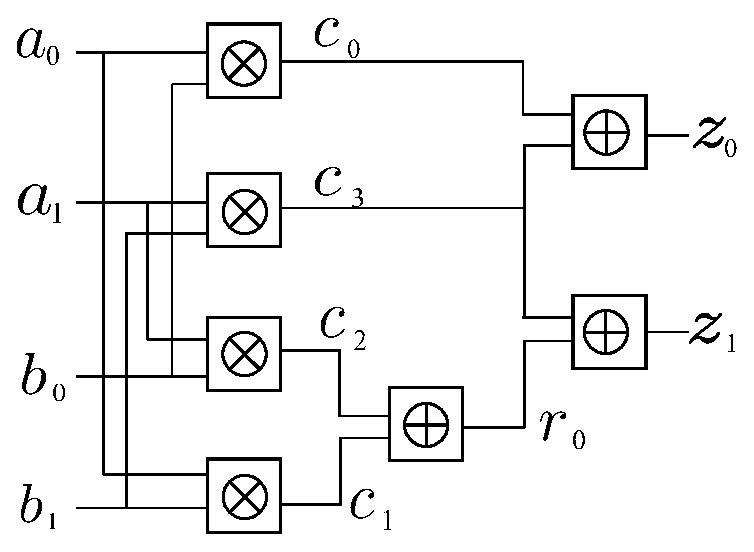
\includegraphics[scale=0.3]{../figures/2bitmultiplier.eps}
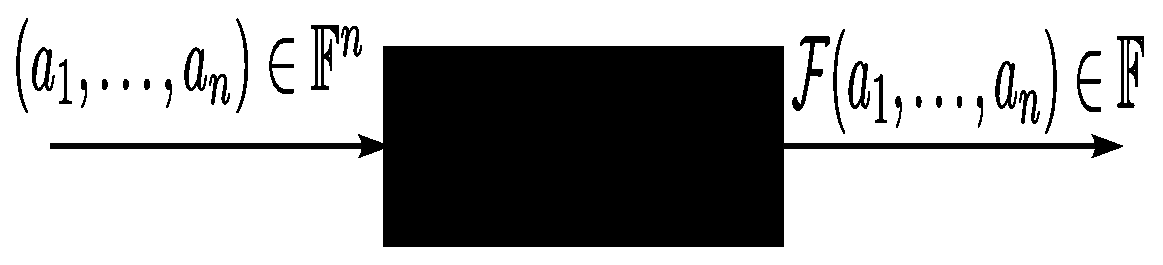
\includegraphics[scale=0.35]{../blackbox.eps}
}
\caption{The black-box or the algebraic circuit representation.}
\label{fig:blackbox}
\end{figure}

Let $\F$ be a multivariate polynomial in $n$ variables $\{x_1, \dots,
x_n\}$, with $t$ non-zero terms ($0 < t < T$), represented with a
black-box $B$. On input $(x_1, \dots, x_n)$,
the black-box evaluates $y_i = \F(x_1, \dots, x_n)$. Given also a
degree bound $d$ on $\F$, the goal is to interpolate the polynomial
$\F$ with a minimum number of {\it probes} to the black-box. The early
work of Zippel \cite{zippel:interpolate} and
Ben-Or/Tiwari \cite{ben-or-tiwari:interpolate} require $O(ndt)$ and
$O(T \log n)$ probes, respectively, to the black-box. These bounds
have since been improved significantly; the recent algorithm of
\cite{monagan:interpolate} interpolates with $O(nt)$ probes.  

Our problem falls into the category of {\it dense} interpolation, as
we require a polynomial that describes the function at each of the $q$
points of the field $\Fq$. Newton's dense interpolation technique,
with the black-box model, bounds the number of probes by $(d+1)^n$ ---
which  exhibits very high complexity. In the logic synthesis area, the
work of \cite{zilic:interpolate} investigates dense interpolation. Due
to the inherent high-complexity, their approach is feasible only for
applications over small fields, {\it e.g.} computing  Reed-Muller
forms for multi-valued logic.  

We can also employ the black-box model by replacing the black-box
(algebraic circuit) by the given circuit $C$; then every {\it probe}
of the black-box would correspond to a {\it simulation of the
  circuit}. As we desire a polynomial representation of the entire
function, exhaustive simulation would be required, which is
infeasible. Therefore, we propose a {\it symbolic approach} to
polynomial interpolation from a circuit using the Gr\"obner basis
computation. 
%It can be shown that the computational complexity of
%computing a Gr\"obner basis for our problem, in the worst case, is
%$q^{O(n)}$, where $q = 2^k$, $k$ is the datapath width and $n$ is the
%number of variables in the circuit.  

\section{Galois Fields, Polynomial Functions \& Hardware Design}
\label{sec:prelimgf}
%\vspace{-0.035in}

%% We briefly describe the relevant concepts related to Galois fields
%% $\Fkk$; for more details, interested readers may refer to the textbook 
%% \cite{galois_field:mceliece}. 
%% %to put the complexity of the verification problem in perspective, 
%% %to shed some light on the complexity of our design verification, 
%% We also review some VLSI architectures used for Galois field
%% computations \cite{mastro:phd} \cite{acar:1998} \cite{wu:2002}
%% \cite{Knezevic:2008} \cite{eccld} \cite{ecc163}. In our experiments,
%% we have verified custom designs based on these architectures. 

%%%%%%%%%%%%%%%%%%%%%%%%%%%%%%%%%%%%%%%%%%%%%%%%%%%%%%%%%%%%%%%%%%%%%%%%%%%%
%% %\begin{Definition}
%% A finite field, also called a {\bf Galois field}, denoted by $F_q$, is
%% a set of $q$ elements, including two distinguished elements 0 and 1,
%% along with operations $'+'$ and $'\cdot'$ (addition and
%% multiplication) that satisfy the following properties: 
%% \begin{itemize}
%% \item ($F_q, +, 0$) forms an Abelian group.

%% % \begin{itemize}
%% % \item  Closure: $\forall a, b \in F_q, a + b \in F_q$.
%% % \item Associativity: $\forall a, b, c \in F_q, a+(b+c)=(a+b)+c$.
%% % \item Commutativity: $\forall a, b \in F_q, a+b=b+a$.
%% % \item Additive Identity: $\forall a \in F_q, a+0=a$. 
%% % \item Additive Inverse: $\forall a \in F_q$, there is an additive
%% %   inverse element $-a \in F_q$ such that $a+(-a)=0$. 
%% %\end{itemize}

%% \item ($F_q, +, \cdot, 0, 1$) forms a commutative ring with unity.
%% % \begin{itemize}
%% % \item Multiplication closure: $\forall a, b \in F_q, a \cdot b \in
%% %   F_q$.
%% % \item Multiplication Associativity: $\forall a, b, c \in F_q, a \cdot
%% %   (b \cdot c)=(a \cdot b)\cdot c$.  
%% % \item Multiplication Commutativity: $\forall a, b \in F_q, a \cdot b=b \cdot a$. 
%% % \item Multiplication Identity: $\forall a \in F_q, a\cdot 1=a$. 
%% % \item Distributivity: $\forall a, b, c \in F_q, a \cdot (b+c)=(a
%% % \cdot b)+(a \cdot c)$. 
%% % \end{itemize}

%% \item Every non-zero element in $F_q$ has a   multiplicative inverse:
%%   $\forall a \in F_q - \{0\}, \exists a^{-1} \in F_q$ such that $a \cdot
%%   a^{-1}=1$. 

%% \item The number of elements $q$ of the finite field is a
%%   power of a prime integer, i.e. $q = p^k, k \geq 1, p=$ prime. 

%% \end{itemize}
%% %\end{Definition}

A Galois field $\Fq$ is a field with a finite number of elements. The
number of elements $q$ of the field is a power of a prime integer ---
i.e. $q = p^k$, where $p$ is a prime integer, and $k \geq 1$
\cite{galois_field:mceliece}. 
%Galois fields are denoted as ${\mathbb{F}}_{q}$ and also $GF(q
%=p^k)$. 
We are interested in fields where $p = 2$ and $k >1$ --- i.e. {\it
  binary Galois extension   fields} $\mathbb{F}_{2^k}$ --- as they are
widely employed in hardware implementations of cryptography
primitives.  

To construct ${\mathbb{F}}_{2^k}$, we take the polynomial ring
${\mathbb{F}}_2[x]$, where ${\mathbb{F}}_{2} = \{0, 1\}$, and an
irreducible  polynomial $P(x) \in {\mathbb{F}}_2[x]$ of degree $k$, and
construct ${\mathbb{F}}_{2^k}$ as ${\mathbb{F}}_2[x] \pmod{   P(x)}$. As a
result, all field operations are performed 
modulo the irreducible polynomial $P(x)$ and the coefficients are
reduced modulo $p=2$. %=2$; due to which $-1 = +1$ over $\Fkk$. 
Any element $A \in {\mathbb{F}}_{2^k}$ can be represented in polynomial
form as $A = a_0 +  a_1 \alpha + \dots + a_{k-1} \alpha^{k-1}$, where
$a_i \in {\mathbb{F}}_2, i = 0, \dots, k-1$, and $\alpha$ is the root of
the irreducible polynomial, {\it i.e.} $P(\alpha)=0$. 
%The field
%$\Fkk$ can therefore be construed as a $k$-dimensional vector space
%over ${\mathbb{F}}_2$.

%For
%example, $\mathbb{F}_{16} =  \mathbb{F}_2[x] \pmod{ x^4 + x + 1}$. 

%% \debug{
%% The {\it characteristic} of any finite field with
%% unity element $1$ is the least integer $n$ such that $1 + \dots + 1$
%% {\it (n times)} $= 0$. The characteristic of fields of the type
%% ${\mathbb{F}}_{p^k}$ %{\mathbb{F}}_p[x] \pmod{ P(x)}$ 
%% is the prime integer $p$. Since in our
%% case $p = 2$, all fields of the type $\Fkk$, for any given $k$, have 
%% characteristic 2. As a result, all field operations are performed
%% modulo the irreducible polynomial $P(x)$ and the coefficients are
%% reduced modulo $p=2$; due to which $-1 = +1$ over $\Fkk$. 
%% }

%% Any element $A \in \mathbb{F}_{2^k}$ can be represented in polynomial
%% form as $A = a_0 +  a_1 \alpha + \dots + a_{k-1} \alpha^{k-1}$, where
%% $a_i \in \mathbb{F}_2, i = 0, \dots, k-1$, and $\alpha$ is the root of
%% the irreducible polynomial, {\it i.e.} $P(\alpha)=0$. The field
%% $\Fkk$ can therefore be construed as a $k$-dimensional vector space
%% over $\mathbb{F}_2$.



\begin{Example}\label{ex:1}
{\it
Let us construct ${\mathbb{F}}_{2^4}$ as ${\mathbb{F}}_2[x] \pmod{
  P(x)}$, where $P(x)=x^4+x^3+1 \in {\mathbb{F}}_2[x]$ is an
irreducible polynomial of degree $k =4$. Let $\alpha$ be the root of
$P(x)$, i.e. $P(\alpha)=0$.  Any element $A \in {\mathbb{F}}_2[x]
\pmod{ x^4 + x^3 + 1}$ has a representation of the type: $A = a_3 x^3
+ a_2 x^2 +  a_1 x + a_0$ where the coefficients $a_3, \dots, a_0$ are
in ${\mathbb{F}}_2 = \{0, 1\}$. Since there are only 16 such
polynomials, we obtain 16 elements in the field
${\mathbb{F}}_{16}$. Each element in can then be viewed as a 4-bit
vector over ${\mathbb{F}}_2$: ${\mathbb{F}}_{16}=\{(0000),(0001),
\dots (1110),(1111)\}$.  Each element also has an exponential
representation; all three representations are shown in Table
\ref{tab:gfelement}. For example, consider the element $\alpha^{12}$.
Computing $\alpha^{12} \pmod{ \alpha^4+\alpha^3+1} = \alpha + 1
= (0011)$; hence we have the three equivalent representations. 
}

\vspace{-0.1in}
\begin{table}[h]
\begin{center}
{\tiny
\caption{Bit-vector, Exponential and Polynomial representation of
elements in  ${\mathbb{F}}_{2^4} = {\mathbb{F}}_2[x]
\pmod{x^4+x^3+1}$}\label{tab:gfelement}  
\begin{tabular}{|c|c|c||c|c|c|} 
\hline
$a_3a_2a_1a_0$ & Exponential & Polynomial     &$a_3a_2a_1a_0$ & Exponential & Polynomial  \\
\hline
$0000$        & $0$         & $0$            & $1000$ & $\alpha^3$ &  $\alpha^3$\\
\hline
$0001$        & $1$         & $1$            & $1001$ & $\alpha^4$ & $\alpha^3 + 1$\\
\hline
$0010$        & $\alpha$    & $\alpha$       & $1010$ & $\alpha^{10}$&$\alpha^3 + \alpha$  \\
\hline
$0011$        & $\alpha^{12}$& $\alpha + 1$   & $1011$ & $\alpha^5$ & $\alpha^3+\alpha+1$\\
\hline
$0100$        & $\alpha^2$  & $\alpha^2$     &  $1100$ & $\alpha^{14}$ & $\alpha^3 + \alpha^2$\\
\hline
$0101$        & $\alpha^9$   &$\alpha^2 + 1$ & $1101$  &$\alpha^{11}$  & $\alpha^3+\alpha^2+1$\\
\hline
$0110$        & $\alpha^{13}$& $\alpha^2 + \alpha$ & $1110$ & $\alpha^8$& $\alpha^3+\alpha^2+\alpha$\\
\hline
$0111$        &$\alpha^7 $ & $\alpha^2+\alpha+1$ & $1111$ &$\alpha^6$ & $\alpha^3+\alpha^2+\alpha+1$\\
\hline
\end{tabular}
}
\end{center}
\end{table}
\end{Example}




%%%%%%%%%
{\bf Polynomial Functions $f: \Fkk \rightarrow \Fkk$:} 
Arbitrary mappings among $k$-bit vectors can be constructed; each such
mapping generates a function $f: \B^k \rightarrow \B^k$. 
%. Since every
%$k$-bit vector can be construed as an element in $\Fkk$ (as shown in
%the above example), every such function corresponds to a function over
Every such function is also a polynomial function over Galois fields:
$f: \Fkk \rightarrow \Fkk$.  

\begin{Theorem}
From \cite{ff:1997}: 
Any  function $f: \Fq \to \Fq$ is a polynomial function
over $\Fq$, that is there exists a polynomial $\F \in \Fq [x]$ such
  that $f(a) = \F(a)$, for all $a \in \Fq$. 
\end{Theorem}

By analyzing $f$ over each of the $q$ points, one can apply
{\bf Langrange's interpolation formula} and interpolate a polynomial
$\F(x) = \sum_{k=1} ^q  \frac{ \prod_{i \neq k}  (x -x_i)}{\prod_{i \neq k}
  (x_k -x_i)} \cdot f(x_k)$, which is a polynomial of degree at 
most $q-1$ in $x$. One can easily see that $\F(a)=f(a)$ for all $a \in
\Fq$, and $\F(x)$ is therefore the polynomial function representation
of $f$. 

%% \begin{Example} {\it
%% Let $A = \{a_2, a_1, a_0\}$ and $Y = \{y_2, y_1,
%% y_0\}$ be 3-bit vectors.  Consider the function $Y[2:0] = A[2:0]
%% >> 1$, i.e. a {\bf bit-vector right shift} operation on $A$. 
%% The function maps as follows:

%% \begin{center}
%% {\small
%% \begin{tabular}{c|ccc|c||c|ccc|c}
%% $\{a_2a_1a_0\}$  & $A$ &$\rightarrow$& $\{y_2y_1y_0\}$ &$Y$ &
%%   $\{a_2a_1a_0\}$  &$A$&$\rightarrow$& $\{y_2y_1y_0\}$ &$Y$\\
%% \hline
%% 000  &0 &$\rightarrow$& 000 & 0 & 100  &$\alpha^2$ &$\rightarrow$& 010 &  $\alpha$ \\
%% 001  &1 &$\rightarrow$& 000 & 0 & 101  &$\alpha^2 + 1$ &$\rightarrow$&010 & $\alpha$ \\
%% 010  &$\alpha$ & $\rightarrow$ & 001& 1 & 110  &$\alpha^2 + \alpha$&$\rightarrow$& 011 &$\alpha + 1$ \\   
%% 011  &$\alpha + 1$ &$\rightarrow$& 001 &1 & 111& $\alpha^2 + \alpha + 1$ &$\rightarrow$& 011 &$\alpha + 1$\\
%% \hline
%% \end {tabular}
%% }
%% \end{center}

%% If we model this function as $f: {\mathbb{Z}}_{8} \rightarrow
%% {\mathbb{Z}}_{8}$, then using the results of \cite{singmaster}
%% \cite{chen_95} \cite{chen_96}, we deduce that this function is not a
%% polynomial function over ${\mathbb{Z}}_{8}$. However, applying
%% Largange's interpolation formula over ${\mathbb{F}}_{2^3}$, we obtain
%% the following polynomial function representation, $Y =
%% (\alpha^2+1)A^4+(\alpha^2+1)A^2$, where $P(\alpha) = \alpha^3 +
%% \alpha + 1 = 0$. 
%% }
%% \end{Example}

An important property of Galois fields is that for all elements $A \in
{\mathbb{F}}_q, A^q = A$, and hence $A^q - A =  0.$ Therefore, the
polynomial $x^q -x$ {\it vanishes} on all points in
$\Fq$. Consequently, any polynomial $\F(X)$ can be reduced $\pmod{ X^q
  - X}$ to obtain a canonical representation $\F(X) \pmod{X^q - X}$
with degree at most $q-1$. 
%Such {\it vanishing polynomials} will form
%an important part of our formulation.  

\begin{Definition}
Any function $f: \Fq^d \to \Fq$ has a unique canonical representation
(UCR) as polynomial $\F \in \Fq[x_1,\dots, x_d]$ such that all its 
nonzero monomials are of the form $x_1^{i_1}\cdots x_d^{i_d}$ where $0
\leq i_j \leq q-1$, for all $j=1, \ldots d$.
\end{Definition}


\subsection{Hardware Implementations of Galois Field Arithmetic}
% Operations Over $\mathbb{F}_{2^k}$}

{\bf Point Addition over Elliptic Curves:} The main operations of
encryption, decryption and authentication in elliptic curve
cryptography (ECC) rely on {\it point additions} and {\it doubling}
operations on elliptic curves designed over Galois fields. 
%Point multiplication involves a series of addition and doubling of
%points on the elliptic curve. % -- this, in turn, requires finite
%field multiplications.  
%A drawback of traditional approaches is that they require
%point multiplication is that each point addition and doubling 
In general, this requires computation of multiplicative inverses over
the field - which is expensive. Modern approaches represent
the points in projective coordinate systems, {\it e.g.}, the
L$\acute{o}$pez-Dahab (LD) projective coordinate \cite{eccld},
%\cite{ecc:software},
which eliminates the need for multiplicative inverses and improves the
efficiency of these operations. 

%%%

%% \begin{Example}
%% {\it 
%% Consider point addition in L$\acute{o}$pez-Dahab (LD) projective
%% coordinate. Given an elliptic curve: $Y^2 + XYZ = X^3Z + aX^2Z^2 +
%% bZ^4$ over $\mathbb{F}_{2^k}$,   where $X,Y,Z$ are $k$-bit vectors
%% that are elements in $\mathbb{F}_{2^k}$ and similarly, $a, b$ are
%% constants from the field.   Let ($X_3$, $Y_3$, $Z_3$) = ($X_1$, $Y_1$,
%% $Z_1$) + ($X_2$, $Y_2$, $1$)  represent point addition over the
%% elliptic curve.  Then $X_3$, $Y_3$, $Z_3$ can be computed as follows: 

%% \begin{align*}
%% A &= Y_2 \cdot Z_1^2 + Y_1 \\
%% B &= X_2 \cdot Z_1 + X_1 \\
%% C &= Z_1 \cdot B \\
%% D &= B^2 \cdot(C + a Z_1^2) \\
%% Z_3 &= C^2 \\
%% E &= A \cdot C  \\
%% X_3 &= A^2 + D + E  \\
%% F &= X_3 + X_2 \cdot Z_3 \\
%% G &= X_3 + Y_2\cdot Z_3 \\
%% Y_3 &= E\cdot F + Z_3 \cdot G \\
%% \end{align*}
%% }
%% \end{Example}

\begin{Example}
{\it 
Consider point doubling in LD projective coordinate system. Given an
elliptic curve: $Y^2 + XYZ = X^3Z + aX^2Z^2 + bZ^4$.  
Let  ($X_3$, $Y_3$, $Z_3$) = 2($X_1$, $Y_1$, $Z_1$), then $X_3, Y_3,
Z_3$ can be computed as: $X_3 = X_1^4 + b \cdot Z_1^4; ~~Z_3 = X_1^2
\cdot Z_1^2; ~~Y_3 = b Z_1^4 \cdot Z_3 + X_3 \cdot (aZ_3 + Y_1^2 +
bZ_1^4 )$. 
}
\end{Example}

The multiplication and iterative squaring operations in the above
computation are usually implemented using custom-designed Galois field
multipliers, such as the Mastrovito \cite{mastro:1989}, Montgomery
\cite{acar:1998}, Barrett multipliers \cite{Knezevic:2008}, or
composite-field multipliers \cite{cfmulti:1996} --- which are, in
turn, hierarchically designed.  
For example, Montgomery reduction (MR)
computes: $MR(A,B)=A\cdot B \cdot R^{-1} \pmod {P(x)}$, 
where $A,B$ are $k$-bit inputs, $R$ is suitably chosen as
$R={\alpha}^k$, $R^{-1}$ is multiplicative inverse of $R$ in
${\mathbb{F}}_{2^k}$, and $P(x)$ is the irreducible polynomial.
Since Montgomery reduction cannot directly compute $A\cdot B \pmod
{P(x)}$, we need to pre-compute $A\cdot R$ and $B\cdot R$, as shown in
Figure \ref{fig:mm4}.   

\begin{figure}[hbt]
	\begin{center}
	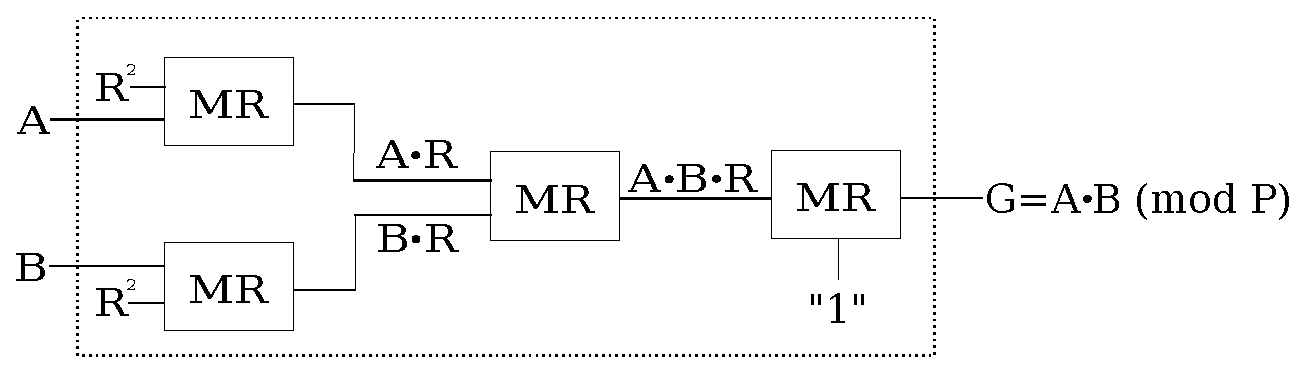
\includegraphics[scale=0.4]{../new_mmcircuit.eps}
	\end{center}
	\caption{{\it Montgomery} multiplication over $\mathbb{F}_{2^k}$
          using four Montgomery reductions.}
	\label{fig:mm4}
\end{figure}

Given a hierarchically designed Montgomery multiplier, we will first
extract polynomials $AR, BR, ABR$ from the sub-circuit blocks. By
analyzing the interconnection of these sub-circuits at word-level, we
can then apply our approach at a higher-level, to extract the function
of the entire circuit. Performing such operations hierarchically, we
will apply our approach to reverse-engineer point-addition circuits
designed using a variety of such Galois field adder and multiplier
circuits.  

\section{Computer Algebra Preliminaries}
\label{sec:ideals}

%We review basic commutative algebra concepts related
%to ideals, varieties, Nullstellensatz and Gr\"obner bases, and their 
%application over Galois fields; the material is referred from
%\cite{ideals:book} \cite{gb_book} and \cite{gao:gf-gb-ms}. 

We denote a Galois field of $q$ elements by $\Fq$, where $q = 2^k$ in
our case. Let $\Fq[x_1,\dots, x_d]$ be
the polynomial ring over $\Fq$ with indeterminates $x_1, \dots, 
x_d$. A {\it monomial} in variables $x_1, \cdots, x_d$ is a product of
the form $X = x_1^{\alpha_{1}}\cdot x_2^{\alpha_{2}}\cdots
x_d^{\alpha_{d}}$, where $\alpha_i \geq 0, i\in \{1, \dots, d\}$. A
{\it polynomial} $f \in \Fq[x_1,\dots, x_d], f\neq 0$, is 
written as a finite sum of terms $f = c_1 X_1 + c_2 X_2 + \dots + c_t
X_t$.  Here $c_1, \dots, c_t$ are coefficients and $X_1, \dots, X_t$
are monomials. To systematically manipulate the polynomials, a {\it
  monomial  ordering} $>$ is imposed such that $X_1 > X_2 > \dots >
X_t$. 
%It is a  well-ordering on the set of all monomials such that
%multiplication with a monomial preserves the
%ordering\footnote{Lexicographic ({\it     lex}), degree-lexicographic
%  ({\it deglex}), degree-reverse-lexicographic ({\it degrevlex}) are
%  examples of monomial orderings.}. 
Subject to such an ordering, $lt(f) = c_1 X_1,  ~lm(f) = X_1, ~lc(f) =
c_1$, are the {\it leading   term}, {\it  leading monomial} and {\it
  leading coefficient} of $f$, respectively. Similarly, tail($f$) =
$c_2X_2 + \dots + c_t X_t$. Division of a polynomial $f$ by polynomial
$g$ gives remainder polynomial $r$, denoted $f \xrightarrow{g}_+ r$.
Similarly, $f$ can be reduced (divided) w.r.t. a set of polynomials
$F = \{f_1, \dots, f_s\}$ to obtain a remainder $r$, denoted $f
\stackrel{F} {\textstyle \longrightarrow}_+ r$, such that no term in
$r$ is divisible by the leading term of any polynomial in $F$.  

%{\bf Polynomial reduction:} Let $f, g$ be polynomials. If a non-zero
%term $cX$ of $f$ is divisible by the leading term of $g$, then we say
%that $f$ {\it reduces} to $r$ modulo $g$, denoted $f
%\stackrel{g}{\textstyle\longrightarrow} r$, where $r = f - {cX   \over
%  lt(g)} \cdot g$. 

{\bf Ideals and varieties:} An {\it ideal} $J$ generated by
polynomials $f_1, \dots, f_s \in \Fq[x_1,\dots, x_d]$ is:
$J = \langle f_1, \dots, f_s \rangle = \{\sum_{i=1}^{s}
h_i\cdot f_i: ~h_i \in \mathbb{F}[x_1,\dots,  x_d]\}.$  The
polynomials $f_1, \dots, f_s$ form the basis or generators of
$J$. 

Let $\mathbf{a} = (a_1, \dots, a_d) \in \Fq^d$ be a point, and
$f \in \Fq[x_1,\dots, x_d]$ be a polynomial. We say that $f$
{\it vanishes} on $\mathbf{a}$ if $f(\mathbf{a}) = 0$. 
For any ideal $J = \langle f_1, \dots, f_s \rangle \subseteq
\Fq[x_1,\dots, x_d]$, the {\it affine variety} of $J$ over
$\Fq$ is:
$V(J) = \{\mathbf{a} \in \mathbb{F}^d: \forall f \in
J, f(\mathbf{a}) = 0\}.$ In other words, the variety corresponds to
the set of all solutions to $f_1 = \dots f_s = 0$. 
%If $J = \langle
%f_1, \dots, f_s \rangle = \langle g_1, \dots, g_t \rangle$, then $V(J)
%= V(f_1, \dots, f_s) = V(g_1, \dots, g_t)$. 

%%%% Florian says: I_{\mathbb{F}}(V)....


%\begin{Definition}
For any subset $V$ of $\Fq^d$, the ideal of polynomials that
vanish on $V$, called the {\it vanishing ideal of $V$}, is defined as: 
$I(V) = \{f\in \Fq[x_1,\dots, x_d]: \forall
\mathbf{a} \in V, f(\mathbf{a}) = 0\}.$
%\end{Definition}

\begin{Proposition}
\label{prop:finIV}
If a polynomial $f$ vanishes on a variety $V$, then $f \in I(V)$. 
\end{Proposition}


%% \vspace{-0.1in}
%% \subsection{Radicals and Nullstellensatz}
%% \begin{Definition}
%% \label{radical}
%% Let $J \subset \mathbb{F}[x_1,\dots, x_d]$ be an ideal. The {\it
%%   radical of $J$} is defined as $\sqrt{J} = \{f \in
%% \mathbb{F}[x_1,\dots, x_d]: \exists m \in \mathbb{N}, f^m \in
%% J\}$. 
%% \end{Definition}

%% When $J = \sqrt J$, then $J$ is said to be a {\it radical
%%   ideal}. Moreover, $I(V)$ is a radical ideal. The Strong 
%% Nullstellensatz establishes the correspondence between radical ideals 
%% and varieties.  

%% \begin{Theorem}
%% {\it Strong Nullstellensatz} \cite{gb_book}:  
%% Let $\mathbb{F}$ be an algebraically closed field, and let $J$
%% be an ideal in $\mathbb{F}[x_1,\dots, x_d]$. Then we have $I(V(J)) =
%% \sqrt{J}$. 
%% \end{Theorem}

%% We are concerned with Galois fields, which are not algebraically
%% closed. When a field $\mathbb{F}$ is not algebraically closed, then
%% the above result can be suitably applied over the algebraic closure of
%% $\mathbb{F}$.    

%% %%%% reinforce I_{\mathbb{F}}(---) 

%% \begin{Corollary}
%% \label{cor:nullsatz}
%% Let $\mathbb{F}$ be an arbitrary field and $J$ be an ideal in
%% $\mathbb{F}[x_1,\dots, x_d]$. Let $\overline{\mathbb{F}}$ denote the
%% algebraic closure of $\mathbb{F}$, and let
%% $V_{\overline{\mathbb{F}}}(J)$ denote the variety of $J$ over
%% $\overline{\mathbb{F}}$. Then $I_{\mathbb{F}}(V_{\overline{\mathbb{F}}}(J)) =
%% \sqrt{J}$.     
%% \end{Corollary}


\subsection{Strong Nullstellensatz over Galois Fields}

Our problem formulation is derived from Nullstellensatz, which admits
a special form over Galois fields. We state the following results of
Nullstellensatz over Galois fields, proofs of which can be found in
\cite{gao:gf-gb-ms}.   

%\begin{Proposition}
Let ${\mathbb{F}}_q$ be a Galois field of $q$ elements. For all elements
$A \in \Fq$, we have $A^q - A = 0$. Therefore, for a polynomial $x^q -
x$, we have $V(x^q - x) = \Fq$.
%\end{Proposition}
The polynomials of the form $\{x^q - x\}$ are called the {\it
  vanishing polynomials} of the field. Let $F_0 = \{x_1^q - x_1,
\dots, ~x_d^q - x_d\}$, then $J_0 = \langle x_1^q - x_1, \dots, x_d^q
- x_d\rangle$ is the ideal of all vanishing polynomials in
$\mathbb{F}_q[x_1,\dots,   x_d]$. Below, we use the concept of sum of
ideals: given ideals $I_1 = \langle f_1, \dots, f_s \rangle$ and $I_2
= \langle g_1, \dots, g_t \rangle$, then ideal $I_1 + I_2 = \langle
f_1, \dots, f_s, g_1, \dots, g_t\rangle$. 

%% \begin{Lemma}
%% \label{lemma:radical}
%% From \cite{gao:gf-gb-ms}: For any ideal $J \subseteq
%% \mathbb{F}_q[x_1,\dots, x_d]$, $J + J_0 = J + \langle x_1^q - x_1,
%% \dots, ~x_d^q - x_d\rangle$ is radical. In other words, $\sqrt{J +
%%   J_0} = J + J_0$. 
%% \end{Lemma}

%% The above is a very powerful result, as it implies that any ideal $J
%% \in \Fq[x_1, \dots, x_d]$ can be easily turned into a radical ideal by
%% adding $J_0$, without changing the zero-set $V(J)$ over $\Fq$. And,
%% based on the above, the following result can be easily deduced:

\begin{Theorem} %\cite{gao:gf-gb-ms}
\label{thm:strong-nullsatz-fq}
{\it Strong Nullstellensatz over $\Fq$:} For any Galois field $\Fq$,
let $J \subseteq \Fq[x_1,\dots,   x_d]$ be an ideal, and let 
$J_0 = \langle x_1^q - x_1, \dots, x_d^q - x_d\rangle$ be
the ideal of all vanishing polynomials. Let $V_{\Fq}(J)$ denote the
variety of $J$ over $\Fq$.  Then, $I(V_{\Fq}(J)) = J + J_0 = J +
\langle  x_1^q - x_1, \dots, ~x_d^q - x_d\rangle$.  
\end{Theorem}


%% \begin{proof}
%% Let $\overline{{\mathbb{F}}_q}$ denote the algebraic closure of
%% $\Fq$. Therefore, $\overline {\mathbb{F}_{q}} \supset
%% \mathbb{F}_{q}$, and we have:

%% \begin{eqnarray}
%% V_{\mathbb{F}_{q}}(J) &= & V_{\overline {\mathbb{F}_{q}}}(J) \cap \mathbb{F}_{q}^d  \nonumber \\
%%                    &= & V_{\overline {\mathbb{F}_{q}}}(J) \cap  V_{\mathbb{F}_{q}}(J_0)  \nonumber \\
%%                    &= & V_{\overline {\mathbb{F}_{q}}}(J) \cap
%% V_{\overline{\mathbb{F}_{q}}}(J_0) \nonumber  \\ 
%%                    &= & V_{\overline {\mathbb{F}_{q}}}(J+J_0) \nonumber
%% \end{eqnarray}

%% Therefore, $I(V_{\Fq}(J)) = I(V_{\overline
%%   {\mathbb{F}_{q}}}(J+J_0)) = \sqrt{J + J_0}$, from Corollary
%% \ref{cor:nullsatz}. Moreover, Lemma \ref{lemma:radical} says that $(J
%% + J_0)$ is radical, so $\sqrt{J + J_0} = J + J_0$. Consequently, we
%% have that $I(V_{\Fq}(J)) = J + J_0$. 
%% \end{proof}

\subsection{Gr\"obner Basis of Ideals} 

An ideal $J$ may have many different generators: it is
possible to have sets of polynomials $F = \{f_1, \dots, f_s\}$ and $G
= \{g_1, \dots, g_t\}$ such that $J = \langle f_1, \dots, f_s \rangle
= \langle g_1, \dots, g_t\rangle$ and $V(J) = V(f_1, \dots, f_s) =
V(g_1, \dots, g_t)$.  Some generating sets are ``better''
than others, i.e. they are a better representation of the ideal. A
{\it Gr\"obner basis} is one such representation which allows to solve
many polynomial decision questions. 

\begin{Definition} \label{def:gb}
$\bf{\left[Gr\ddot{o}bner\ Basis\right]}$ [From \cite{gb_book}] For
a monomial ordering $>$, a set  of non-zero polynomials $G =
\{g_1,g_2,\cdots,g_t\}$ contained in an ideal $J$, is called a
Gr\"{o}bner basis for $J$ $\iff$ 
$\forall f \in J$, $f\neq 0$, there exists $i \in \{1,\cdots, t\}$ such
that $lm(g_i)$ divides $lm(f)$; i.e., $G = GB(J)
\Leftrightarrow\  \forall f \in J : f \neq 0, \exists g_i \in G :
lm(g_i)\mid lm(f)$. 
\end{Definition}

Gr\"obner bases theory 
provides a {\it decision procedure to test for membership in an
ideal}. As a consequence of Definition \ref{def:gb}, the set $G$ is a
Gr\"obner basis of ideal $J$, if and only if for all $f \in J$,
dividing $f$ by polynomials of $G$ gives  0 remainder:  $G = GB(J)
\iff \forall f\in J, f \stackrel{G}{\textstyle\longrightarrow}_+ 0$. 

Buchberger's algorithm \cite{buchberger_thesis},
shown in Algorithm \ref{alg:gb},  computes a Gr\"obner
basis over a field. Given polynomials $F = \{f_1, \dots, f_s\}$, 
the algorithm computes the Gr\"obner basis $G = \{g_1, \dots, 
g_t\}$.
% such that ideal $I = \langle f_1, \dots, f_s\rangle = \langle g_1,
% \dots, g_t\rangle$. 
In the algorithm,  

\begin{equation}
       Spoly(f,g)=\frac{L}{lt(f)}\cdot f - \frac{L}{lt(g)}\cdot g \nonumber
      \label{eqn:spoly}
\end{equation}
where $L = \text{LCM}(lm(f), lm(g))$, where $lm(f)$ is the leading
monomial of $f$, and $lt(f)$ is the leading term of $f$. 


\begin{algorithm}[hbt]
\SetAlgoNoLine
 \KwIn{$F = \{f_1, \dots, f_s\}$}
 \KwOut{$G = \{g_1,\dots ,g_t\}$\\} %, a Gr\"{o}bner basis
  $G:= F$\;
  \Repeat{$G = G'$}
  {
  	$G' := G$\;
  	\For{ each pair $\{f, g\}, f \neq g$ in $G'$} 
	{
		$Spoly(f, g) \stackrel{G'}{\textstyle\longrightarrow}_+r$ \;
		\If{$r \neq 0$}
		{
			$G:= G \cup \{r\}$ \;
		}
	}
   }
\caption {Buchberger's Algorithm}\label{alg:gb}
\end{algorithm}

We now describe our word-level abstraction problem formulation using
Strong Nullstellensatz over $\Fkk$, and its solution using Gr\"obner
bases and Buchberger's algorithm.

%% For Gr\"obner basis computation, a monomial (term) ordering is
%%   fixed to ensure that polynomials are manipulated in a consistent
%%   manner. 
%% %Conventionally, the lexicographic 
%% %(lex), degree-lexicographic (deg-lex) and degree-reverse-lexicographic
%% %(degrevlex) are used. 
%% Buchberger's algorithm then takes pairs of polynomials in the basis
%% and combines them into ``$S$-polynomials'' to cancel leading terms. An
%% $S$-polynomial is defined as: 
%% \begin{equation}
%%        S(f,g)=\frac{L}{lt(f)}\cdot f - \frac{L}{lt(g)}\cdot g
%%       \label{eqn:spoly}
%% \end{equation}
%% where $L = \text{LCM}(lm(f), lm(g))$, where $lm(f)$ is the leading
%% monomial of $f$, and $lt(f)$ denotes the leading term of $f$. The
%% $S$-polynomial is then reduced (divided) by all elements of $G'$ to a
%% remainder $r$, denoted as 
%% $S(f, g) \stackrel{G'}{\textstyle\longrightarrow}_+r$. 
%% Multivariate polynomial division is used for this reduction step. This
%% process is repeated for all unique pairs of polynomials, including
%% those created by newly added elements, until no new polynomials are
%% generated; ultimately constructing the Gr\"{o}bner basis.

\section{Word-Level Abstraction using Gr\"obner basis}
\label{sec:theory}
We are given a circuit $C$ with $k$-bit inputs and outputs that
performs a polynomial computation $Y = \F(A)$ over $\Fq = \Fkk$. Let
$P(x)$ be the {\it given} irreducible or primitive polynomial used for
field construction, and let $\alpha$ be its root, i.e. $P(\alpha) = 0
$. Note that we do not know the polynomial representation
$\F(A)$ and our objective is to identify (the coefficients of)
$\F(A)$. Let $\{a_0, \dots, a_{k-1}\}$ denote the primary inputs and
let $\{y_0, \dots, y_{k-1}\}$ be the primary outputs of $C$. Then, the
word-level and bit-level correspondences are: 
\begin{equation}
\label{eqn:words}
 A = a_0 + a_1 \alpha + \dots + a_{k-1} \alpha^{k-1}; ~~ Y = y_0 +
y_1 \alpha + \dots + y_{k-1} \alpha^{k-1};
\end{equation}

We analyze the circuit and model all the gate-level Boolean operators
as polynomials in ${\mathbb{F}}_2 \subset \Fkk$. To this set of
Boolean polynomials, we append the polynomials of Eqn
(\ref{eqn:words}) that relate the word-level and bit-level
variables. We model this set of polynomials as $F = \{f_1, \dots,
f_s\}$ over the ring $R = \Fq[x_1, \dots, x_d, Y, A]$. Here $x_1,
\dots, x_d$ denote, collectively, all the bit-level variables of the
circuit --- i.e. primary inputs, primary outputs and the intermediate
circuit variables --- and $Y, A$ the word-level variables. Denote the
generated ideal as $J = \langle F \rangle \subset R$. As $Y = \F(A)$
is a polynomial representation of the circuit, represent this (unknown)
``specification'' as a polynomial $f: Y - \F(A)$, or as $f: Y + \F(A)$
and $-1 = +1$ over $\Fkk$.  

As the circuit $C$ implements the function $f$, clearly $f$ {\it
  agrees with the solutions} to $f_1 = \dots = f_s = 0$. In computer
algebra terminology, this means that $f$ {\it vanishes on the variety} 
$V_{\Fq}(J)$. If $f$ vanishes on $V_{\Fq}(J)$, then $f$ is a member of
the ideal $I(V_{\Fq}(J))$. Strong Nullstellensatz over Galois fields
(Theorem \ref{thm:strong-nullsatz-fq}) tells us that $I(V_{\Fq}(J)) =
J + J_0$, where $J_0 = \langle x_1^q - x_1, \dots, x_d^q - x_d, Y^q -
Y, A^q - A \rangle$ is the ideal of vanishing polynomials in
$R$. Consolidating these results, we deduce that the specification
polynomial $f \in (J+J_0)$. 

If the specification polynomial is known, then the verification
problem can be solved using membership testing of $f$ in the ideal $(J
+ J_0)$ (\cite{lv:date2012} used such a formulation). We will now show
that by computing a Gr\"obner basis of $(J + J_0)$, using a specific
elimination term order, we can also identify the polynomial $f$ which
represents the function implemented by the circuit.


{\bf Reverse-Engineering $f$ from $C$:} The variety $V_{\Fq}(J)$ is
the set of all consistent assignments to the nets (signals) in the
circuit $C$. If we {\it project this variety on the word-level input and
output variables of the circuit $C$, we essentially generate the
function $f$ implemented by the circuit.} Projection of varieties from
$d$-dimensional space $\Fq^d$ onto a lower dimensional subspace
$\Fq^{d-l}$ is equivalent to {\it eliminating $l$ variables} from the
corresponding ideal. 

\begin{Definition}
    ({\bf Elimination Ideal}) From \cite{ideals:book}:  Given
  $J=\langle f_1,\dots,f_s\rangle \subset \Fq[x_1,\dots,x_d]$, the
  $l$th {\bf elimination ideal} $J_l$ is the ideal of
  $\Fq[x_{j+1},\dots,x_d]$ defined by 
    \begin{equation}
        J_l= J \cap \Fq[x_{l+1},\dots,x_d]
    \end{equation}
\end{Definition}

In other words, the $l$th elimination ideal does not contain variables
$x_1,\dots,x_l$, nor do the generators of it.  This can aid in solving
systems of polynomial equations by isolating variables in a set of
constraints, as is the purpose of techniques such as Gaussian
elimination. 
%The generators of a $k$th elimination ideal are such that
%$variables  are not present.
Moreover, Gr\"obner bases may be used to generate an elimination ideal
by using an ``elimination order.''  One such ordering
is a pure lexicographic ordering, which features into a theorem:
%The ideal $I_k$ is spanned by elements which eliminate variables
%$x_1,\dots,x_k$.  This leads to an {\bf elimination theorem} for \Grobner
%bases:
\begin{Theorem} \label{thm:elim}
({\bf Elimination Theorem}) From \cite{ideals:book}: Let $J
  \subset \Fq[x_1,\dots,x_d]$ be an     ideal and let $G$ be a
  Gr\"obner basis of $J$ with respect to a lex ordering where $x_1
  > x_2 > \dots > x_d$.  Then for every $0     \leq l \leq
  d$, the set 
    \begin{equation}
        G_l= G \cap \Fq[x_{l+1},\dots,x_d]
    \end{equation}
    is a Gr\"obner basis of the $l$th elimination ideal $J_l$.
\end{Theorem}

We describe the application of elimination ideals using the following
example, borrowed from \cite{ideals:book}.

\begin{Example}

{\it 
Consider polynomials $f_1: x^2 - y - z - 1; ~~f_2: x - y^2 - z -1; 
~~f_3: x - y - z^2 - 1$ and ideal $J = \langle f_1, f_2, f_3\rangle
\subset {\mathbb{C}}[x, y, z]$. Let us compute a Gr\"obner basis $G$
of $J$ w.r.t. lex term order with $x > y > z$. Then $G = \{g_1, \dots,
g_4\}$ is obtained as: $g_1: x - y - z^2 - 1; ~~g_2: y^2 - y - z^2 - z;
~~g_3: 2yz^2 - z^4 - z^2; ~~g_4: z^6 - 4z^4 - 4z^3 - z^2$. 
Notice that the polynomial $g_4$ contains only the variable $z$, and
it {\bf eliminates} variables $x, y$. Similarly, polynomials $g_2,
g_3, g_4$, contain variables $y, z$ and eliminate $x$. According to
Theorem \ref{thm:elim}, $G_1 = G \cap {\mathbb{C}}[y, z] = \{g_2, g_3,
g_4\}$ and $G_2 = G \cap {\mathbb{C}}[z] = \{g_4\}$ are the Gr\"obner
bases of the $1^{st}$ and $2^{nd}$ elimination ideals of $J$, respectively.
}
\end{Example}

In conclusion, Gr\"obner basis computations w.r.t. pure lexicographic
term orders can be used to eliminate variables from an ideal. The
above example motivates our approach: Since we want to derive a
polynomial representation from a circuit in variables $Y, A$, we can
compute a Gr\"obner basis of $J + J_0$ w.r.t. an elimination order
that eliminates all the ($d$) bit-level variables of the
circuit. Then, the Gr\"obner basis $G_d = G \cap \Fq[x_1, \dots, x_d,
  Y, A]$ of the $d^{th}$ elimination ideal of $(J + J_0)$ will contain
polynomials in only $Y, A$. We now prove that the 
required polynomial representation will be found in $G_d$.
%$Y = \F(A)$
%will be found in $G_d$ and it will be the polynomial representation of
%the function implemented by the circuit.
First, let us formally ``setup'' the abstraction problem:

\begin{Setup}\label{not:abs}
Given a circuit $C$ with $k$-bit inputs and outputs which computes a
polyfunction $f: \Fkk \rightarrow \Fkk$. Let $\{a_0, \dots, a_{k-1}\}$
be the bit-level primary inputs and $\{y_0, \dots, y_{k-1}\}$ be the
primary outputs. Let $A, Y$ denote the word-level input and output
variables of the circuit, respectively, such that $A = a_0 + a_1
\alpha + \dots + a_{k-1}\alpha^{k-1}$ and $Y = y_0 + \dots +
y_{k-1}\alpha^{k-1}$, where $\alpha$ is a primitive element of $\Fkk$. 
Let ${\mathcal{F}}(A)$ be the (unknown) polynomial representation of
the function implemented by the circuit such that $Y =
{\mathcal{F}}(A)$.  

Denote by $x_i, i = 1, \dots, d$ all the Boolean variables of the
circuit -- i.e. the input, output and the intermediate
variables. Let $R = \Fkk[x_i, Y, A: i = 1, \dots d]$ denote the
ring to model the polynomials that describe 
the circuit functionality. Let ideal $J \subset \Fkk[x_i, Y, A: i = 1
  \dots d]$ be generated by the bit-level and word-level polynomials
of the circuit. Let $J_0 = \langle x_i^2-x_i, Y^{2^k} - Y, A^{2^k} - A: i =
1, \dots, d\rangle$ denote the ideal of vanishing polynomials in $R$. 
\hfill$\Box$
\end{Setup}

Now, we will impose the following elimination order used for
abstraction: 

\begin{Definition}
{\bf Abstraction Term Order $>$:} 
%For the given circuit $C$,
%let $x_1, \dots, x_d$ denote all the bit-level variables, and let $Y,
%A$ denote, respectively the word-level output and input
%variables. 
Using the variable order $x_1 > x_2 > \dots > x_d > Y > A$,
impose a lex term order $>$ on the polynomial ring $R = \Fq[x_1,
  \dots, x_d, Y, A]$. This elimination term order $>$ is defined as
the {\bf Abstraction Term Order}. 
\end{Definition}


\begin{Theorem} \label{thm:abs}
{\bf Abstraction Theorem:} Using the setup and notations from Problem
Setup \ref{not:abs} above, compute a Gr\"obner basis $G$ of ideal $(J
+ J_0)$ using the abstraction term order $>$. Then: \\
(i) $G$ must contain the vanishing polynomial $A^q - A$ as the only
polynomial with only $A$ as the support variable;\\
(ii) $G$ must contain a polynomial of the form $Y + {\mathcal{G}}(A)$;
and\\ 
(iii) $Y + {\mathcal{G}}(A)$ is such that $\F(A) = {\mathcal{G}}(A),
\forall A \in \Fq$. In other words, ${\mathcal{G}}(A)$ and $\F(A)$ are
equal as polynomial functions over $\Fq$.
\end{Theorem}

\begin{proof}
(i) $A^q -A$ is a given generator of $J_0$. Variable $A$ is also the
  last variable in the abstraction term order. Moreover, $A$ is an
  input to the circuit, so $A$ is an independent variable which can
  take any and all values in $\Fkk$. As a   result, $G_{d+1} = G \cap
  \Fkk[A] = \{A^q - A\}$.

(ii) Since $f:Y + {\mathcal{F}}(A)$ is a polynomial representation of
  the function of the circuit, $Y + {\mathcal{F}}(A) \in J + J_0$, as
  described above. Therefore, according to the definition of a
  Gr\"obner basis (Definition \ref{def:gb}), the leading term of $Y +
  {\mathcal{F}}(A)$ (which is $Y$) should be divisible by the leading
  term of some polynomial $g_i \in G$. The only way $lt(g_i)$ can
  divide $Y$ is when $lt(g_i) = Y$ itself. Moreover, due to our
  abstraction (lex) term order, $Y > A$, so this polynomial must be
  of the form $Y + {\mathcal{G}}(A)$. 

(iii) As $Y = \F(A)$ represents the function of the circuit, $Y +
  \F(A) \in J + J_0$. Moreover, $V(J + J_0) \subset V(Y + \F(A))$. 
  Project this variety $V(J + J_0)$ onto the co-ordinates
  corresponding to $(A, Y)$. What we obtain is the {\it graph of the
  function} $(A) \mapsto \F(A)$ from $\Fkk \rightarrow \Fkk$. Since $Y
  + {\mathcal{G}}(A)$ is an element of the Gr\"obner basis of $J +
  J_0$, $V(J + J_0) \subset V(Y + {\mathcal{G}}(A))$ too. Therefore,
  $Y = {\mathcal{G}}(A)$ gives the same function as $Y = \F(A)$, for
  all $A \in \Fkk$.
\end{proof}

As a consequence of Theorem \ref{thm:abs}, if we compute a Gr\"obner
basis $G$ of $J + J_0$ using the abstraction term order, we will find
a polynomial of the form $Y + \G(A)$ in the Gr\"obner basis, such that
$Y = \G(A)$ is a polynomial representation of the circuit. However, if
the Gr\"obner basis is not reduced, it is possible to obtain multiple
polynomials in $G$ of the form $Y + \G _1(A), Y + \G _2(A), \dots,$;
all of which correspond to the same function. 

\begin{Corollary}
Computing a {\bf reduced} Gr\"obner basis $G_r$ of $J + J_0$, we
will obtain {\bf one and only one polynomial} in $G_r$ of the form $Y
+ \G(A)$, such that $Y = \G(A)$ is the {\bf unique, minimal,
  canonical} representation of the function $f$ implemented by the
circuit.  
\end{Corollary}

The above results trivially extend to circuits with multiple
word-level input variables $A^1, \dots, A^n$, and the canonical
polynomial representation obtained by computing a reduced Gr\"obner
basis $G_r$ of $J + J_0$ using $>$ is of the form $Y = \F(A^1, \dots,
A^n)$. 

\section{Research to be conducted further....}

{\it Gr\"obner basis Complexity:} To compute a Gr\"obner basis for
$J + J_0$ over $\Fq$, the following result is known \cite{gao:gf-gb-ms}:  

\begin{Theorem}
Let $J = \langle f_1, \dots, f_s, ~x_1^q - x_1, \dots, x_d^q -
x_d\rangle \subset \Fq [x_1, \dots, x_d]$ be an ideal. The time and
space complexity of Buchberger's algorithm to compute a Gr\"obner
basis of $J$ is bounded by $q^{O(d)}$.
 assuming that the length of input $f_1, \dots, f_s$ is dominated by
 $q^{O(d)}$.  
\end{Theorem}

In our case, $q = 2^k$, and when $k$ and $d$ are large, this complexity
may make  verification infeasible. Therefore, I wish to conduct
research to make this approach scalable. Talk about FGLM here, and
maybe show an example corresponding to the same 2-bit multiplier
circuit....... You take it up from here.... 




\section{Preliminary experiments and FGLM}
\label{sec:fglm}

%{\it Gr\"obner basis Complexity:} To compute a Gr\"obner basis for
%$J + J_0$ over $\Fq$, the following result is known \cite{gao:gf-gb-ms}:  

\begin{Theorem}
(From \cite{lv:date2012}:) Let $J + J_0 = \langle f_1, \dots, f_s, ~x_1^q -
  x_1, \dots, x_d^q - x_d\rangle \subset \Fq [x_1, \dots, x_d]$ be an
  ideal. The time and space complexity of Buchberger's algorithm to
  compute a Gr\"obner basis of $J + J_0$ is bounded by $q^{O(d)}$.
 assuming that the length of input $f_1, \dots, f_s$ is dominated by
 $q^{O(d)}$.  
\end{Theorem}

In our case $q = 2^k$, and when $k$ and $d$ are large, this complexity 
makes verification infeasible. The impact of this complexity is clearly
visible in the results of preliminary experiments (TABLE \ref{tab:sT}).
The experiments are conducted with Mastrovito \cite{mastro:1989}
multiplier circuits of various word sizes $k$. Each multiplier
computes the polynomial function  $Y = \F(A,B) = A \cdot B$ over
$\Fkk$, where $Y, A, B$ are $k$-bit vectors. We extract the 
Boolean gate-level operators $J$ and generate vanishing polynomials $J_0$.
Then we compute the Gr\"obner basis of $J + J_0$
with respect to abstraction term order $>$. The computation was performed
using the "slimgb" command in the {\sc Singular'} computer algebra
tool \cite{DGPS}. The resulting Gr\"obner bases contained a polynomial
$Y + A \times B$.  
These experiments were run on a 64-bit Ubuntu OS running on a 2.4GHz 
Intel QuadCore processor with 8Gb of memory. The approach is
infeasible beyond 40-bit datapath size, as the Gr\"obner basis engine
encounters a memory explosion. BDDs cannot be constructed for
any of these circuits. 

%In Elliptic Curve Cryptography, the 
%minimum suggested word-size is 163 bits, as set by the US National Institute 
%for Standards and Technology. Therefore, I wish to conduct research to make 
%this approach scalable.

\begin{table}[h]
{\small
	\begin{center}
	    \caption{Gr\"obner Basis runtime for
              Mastrovito Multipliers in Singular using Abstraction
              Term Order $>$.}\label{tab:sT} 
	    \begin{tabular}{|c|c||c|} 
	        \hline
		Word Size ($k$) & \# Polynomials (\# gates) & Time (minutes)   \\
		\hline
	        $16$	&  $1,871$  & $2.4$ \\
		$24$	&  $3,135$  & $12$  \\
	        $32$	&  $5,549$  & $22.6$ \\
	        $40$	&  $8,587$  & $266$ \\
		$48$	& $12,327$  & NA (Out of Memory) \\
	        \hline
	    \end{tabular}
	\end{center} 
}
\end{table}

{\it Proposed FGLM Approach:} To make this approach scalable, we are
investigating the use of the FGLM algorithm \cite{fglm}. This
algorithm provides a method for converting a Gr\"obner basis in one
term ordering to a  Gr\"obner Basis in another term ordering.
We use this method in conjunction with following result which was
derived and proved in \cite{lv:date2012}: 

\begin{Theorem} \label{thm:top-order}
Let $C$ be any arbitrary combinational circuit. Let $\{x_1, \dots,
x_d\}$ denote the set of all variables (signals) in the circuit,
i.e. the primary input, intermediate and primary output
variables. Perform a {\it reverse topological traversal} of the
circuit and order the variables such that $x_i > x_j$ if $x_i$ appears
earlier in the reverse topological order. Impose a lex term order to
represent each gate as a polynomial $f_i$,
s.t. $f_i = x_i + \text{tail}(f_i)$. Then the set of all polynomials 
$G_1 = \{f_1, \dots, f_s, x_i^q - x_i: i = 1, \dots, d\}$ constitutes
a Gr\"obner basis.
%, as $lt(f_i)$ and $ lt(f_j)$ for $i\neq j$ are relatively prime.
\end{Theorem}



Using the term ordering specified by \cite{lv:date2012}, which we
denote $>_1$,  we can obviate the need to compute a Gr\"obner
basis. Imposing the monomial ordering $>_1$ already makes $G_1$ a
Gr\"obner basis of $J + J_0$. Now we apply the FGLM algorithm to
transform the Gr\"obner basis into another basis w.r.t. the
abstraction ordering $>$.  This new basis will also definitely contain
a polynomial in the form of $Y + \F(A)$ as desired. By using FGLM to
convert the Gr\"obner basis from $>_1$ to $>$, we are hoping to avoid
the complexity presented by computing a Gr\"obner basis over the
abstraction ordering $>$.  


\begin{Example}
\label{ex:myapproach}
{\it
Let us revisit the 2-bit multiplier circuit from Example \ref{ex:twomult}, 
shown in Fig. \ref{fig:mul2bit}. 
 
%\begin{figure}[htb]
%\centerline{
%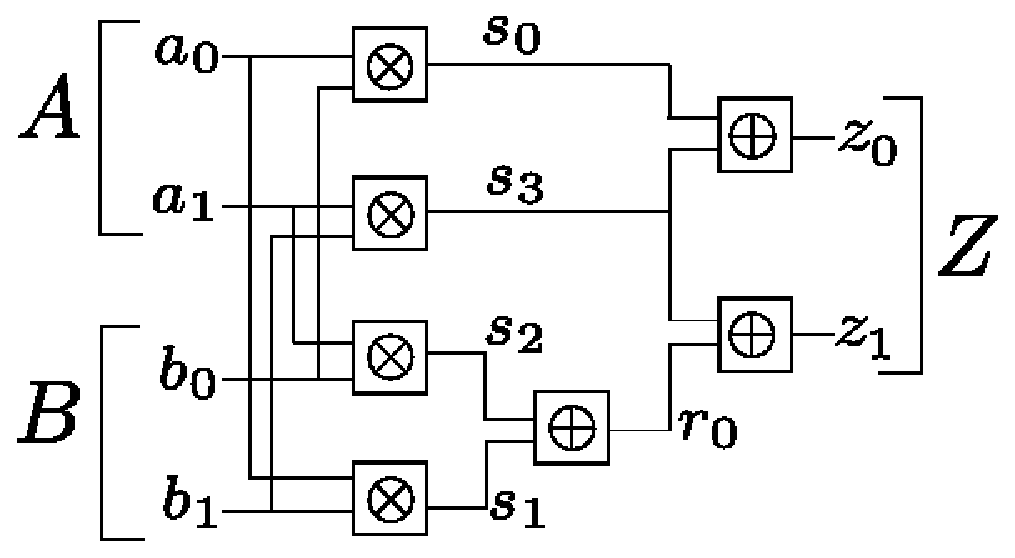
\includegraphics[scale=0.35]{2bitmult.eps}
%}
%\caption{\small A 2-bit Multiplier over ${\mathbb{F}}_{2^2}$. The gate
%  $\otimes$ corresponds to AND-gate, i.e. bit-level multiplication
%  modulo 2. The gate $\oplus$ corresponds to XOR-gate, i.e. addition
%  modulo 2.} 
%\label{fig:mul2bit2}
%\end{figure}
As before, we can describe the functionality of this circuit, $J$, using the
following polynomials: $f_1: Z+z_0+z_1\alpha; ~~f_2: B+b_0+b_1\alpha; ~~f_3: A+a_0+a_1 \alpha
; ~~f_4: s_0+a_0 \cdot b_0; ~~f_5: s_1+a_0 \cdot b_1; ~~f_6:
s_2+a_1 \cdot b_0; ~~f_7: s_3+a_1 \cdot b_1; ~~f_8: r_0+s_1 + s_2;
~~f_9: z_0+s_0 + s_3; ~~f_{10}: z_1 + r_0 + s_3$.
By imposing the monomial order $>_1$, $J+J_0$ is already a Gr\"obner basis, 
where $J_0$ is the ideal of vanishing polynomials of the circuit:
$~~f_{11}: a_0^2+a_0; ~~f_{12}: a_1^2+a_1; ~~f_{13}: b_0^2+b_0;
~~f_{14}: b_1^2+b_1; ~~f_{15}: s_0^2+s_0; ~~f_{16}: s_1^2+s_1;
~~f_{17}: s_2^2+s_2; ~~f_{18}: s_3^2+s_3; ~~f_{19}: r_0^2+r_0;
~~f_{20}: z_0^2+z_0; ~~f_{21}: z_1^2+z_1$. We denote this Gr\"obner
basis as $G_1 = \{f_1, \dots, f_{21}\}$. Using the FGLM algorithm 
("fglm" command in  Singular) we convert $G_1$
from ordering $>_1$ to $G$ with the abstraction term ordering $>$. 
The resulting Gr\"obner basis $G$ contains the 
polynomial $Z \cdot (\alpha+1)+A \cdot B \cdot (\alpha+1)$, 
which can be equivalently reduced to $Z+A \cdot B$.
}
\end{Example}

FGLM exploits concepts from algebraic geometry and sparse linear
algebra to transform the Gr\"obner basis. While a detailed exposition
of FGLM is beyond the scope of this paper, we demonstrate its
operation on the 2-bit multiplier shown in Example
\ref{ex:myapproach}.  

\begin{Example}
\label{ex:approach}
{\it
FGLM begins by taking the least variable in the the abstraction term 
ordering, ($A$ in our case). Starting with $m=0$, it computes $A^m
\xrightarrow{G_1}_+r$. It checks whether the remainder $r$ can be
represented as a linear combination of any remainders calculated thus
far. If so, it adds this  representation to $G$ and moves on to the
next monomial; otherwise it  increments $m$ and repeats $A^m
\xrightarrow{G_1}_+r$ computation. 

\begin{itemize}
\item $A^0 \xrightarrow{G_1}_+ 1$
\item $A^1 \xrightarrow{G_1}_+ a_0+ a_1 \alpha$
\item $A^2 \xrightarrow{G_1}_+ a_0+a_1 \cdot (\alpha+1) $
\item $A^3 \xrightarrow{G_1}_+ a_0 \cdot a_1+a_0+a_1$
\item $A^4 \xrightarrow{G_1}_+ a_0+ a_1 \alpha = A$
\end{itemize}

$A^4$ can be composed of $A$, so $A^4 - A$ is added to $G$. Similarly,
$B^4 - B$ is also added to $G$. Continue to the next variable $Z$ in
the order as we have ``circuit variables'' $> Z > A > B$. 
\begin{itemize}
\item $Z^1 \xrightarrow{G_1}_+ a_0 \cdot b_0+(\alpha) \cdot a_0 \cdot
  b_1+(\alpha) \cdot a_1 \cdot b_0+(\alpha^2) \cdot a_1 \cdot b_1 = 
a_0(b_0 + b_1 \alpha) + a_1\alpha (b_0 + b_1 \alpha) = (a_0 + a_1
\alpha)(b_0 + b_1 \alpha) = A   \cdot B$ 
\end{itemize}
$Z$ is found to be a function of $A$ and $B$, therefore $Z - AB$ is
added to $G$.
}
\end{Example}

FGLM continues to convert the rest of the monomials into the new ordering. However, 
since we are only looking for $Y=\F(A)$ polynomial representation, we
can make this approach even more efficient by restricting the
conversion to only the word-level variables of the circuit. This idea
is currently under development. 

\section{Conclusions}
\label{sec:concl}

This paper has described an approach to derive a word-level, canonical
polynomial representation from combinational circuits using Gr\"obner
bases. Our approach interprets the function of the circuit $f: \B^k
\rightarrow \B^k$ as a polynomial function over Galois fields $f: \Fkk
\rightarrow \Fkk$. By deriving a set of polynomials corresponding to
the circuit (ideal $J + J_0$), and computing its Gr\"obner basis
w.r.t. a specific elimination (abstraction) term order, the canonical
representation of this circuit can be derived. As Gr\"obner basis
computation exhibits high complexity, we are currently investigating
the use of the FGLM algorithm to make our approach scalable. 

\section{Further discussion on Computer Algebra}
\label{sec:moretheory}

Bit level circuit variables including primary inputs/outputs can only take value
within $\Z_2$. They can also be written in functions of other variables and constants.
In computer algebra, circuit variable $a$ can be described as a polynomial, that is
$a = f(x_0, x_1, \dots, x_{n-1}) \in {\mathbb{F}}[x]$. Moreover, circuit variable can
have multiple specifications, they can be written in polynomials and included in an
ideal $I = \{f_0, f_1, \dots, f_k\}$. The varieties of this ideal are possible 
assignments of circuit variable. Similarly for $n$ bits world-level circuit 
variables, the varieties are elements from $\Fkk$. Thus it's convenient to use
ideals and varieties to describle circuit variables. \par

\begin{Definition}
({\bf Sum of Ideals}) If I and J are ideals in $k[x_1, \dots, x_n]$, then the 
{\bf sum} of I and J, denoted I + J, is the set
  \begin{equation}
  I + J = \{f + g : f \in I and g \in J\}.
  \end{equation}
Furthermore, if $I = \langle f_1, \dots, f_r\rangle$ and 
$J = \langle g_1, \dots, g_s\rangle$, then 
$I + J = \langle f_1, \dots, f_r, g_1, \dots, g_s\rangle$.
\end{Definition}

\begin{Definition}
({\bf Product of Ideals}) If I and J are ideals in $k[x_1, \dots, x_n]$, then the
{\bf product} of I and J, denoted $I \cdot J$, is defined to be the ideal generated 
by all polynomials $f \cdot g$ where $f \in I$ and $g \in J$. Furthermore, let
$I = \langle f_1, \dots, f_r\rangle$ and $J = \langle g_1, \dots, g_s\rangle$, then
  \begin{equation}
  I \cdot J = \langle f_ig_j : 1 \leq i \leq r, 1 \leq j \leq s\rangle .
  \end{equation}
\end{Definition}

\begin{Definition}
({\bf Quotient of Ideals}) If I and J are ideals in $k[x_1, \dots, x_n]$, then I:J
is the set
  \begin{equation}
  \{f \in k[x_1, \dots, x_n] : fg \in I \forall g \in J\}
  \end{equation}
and is called the {\bf ideal quotient} of I by J.
\end{Definition}

According to definitions above, it's possible to calculate ideal sum, product and 
quotient based on ideal generators. Additionally conclusion about union, 
intersection and complement of varieties can be attained below: \par

\begin{Theorem}
\label{thm:unionintersect}
If I and J are ideals in $k[x_1, \dots, x_n]$, then ${\bf V}(I + J) = {\bf V}(I)
\bigcap {\bf V}(J)$ and ${\bf V}(I \cdot J) = {\bf V}(I) \bigcup {\bf V}(J)$.
\end{Theorem}

\begin{Theorem}
\label{thm:quotient}
Let V and W be varieties in $\Fkk$. Then ${\bf I}(V) : {\bf I}(W) = 
{\bf I}(V - W)$.
\end{Theorem}

For \ref{thm:quotient}, let $V = \Fkk = {\bf V}(\langle vanishing polynomials
\rangle)$, then $V - W$ is the complementary set of variety $W$.\\

Based on these conclusions it's easy to get a circuit variable's specifications
or possible assignments from the other known information.





\section{Sequential circuits and Finite State Machine}
\label{sec:fsm}
{\bf Introduction to Finite State Machine:}\par
{\bf Symbolic Image Computation:}\par
{\bf Implicit State Enumeration:}\par





\section{Experiments using new approach}
\label{sec:exp}

First example is reachable state enumeration of a 2-bit finite state machine.
Breadth-First-Search traversal (mentioned in \ref{sec:fsm}) is adopted.

\begin{Example}
\label{ex:traversal}
Sample circuit is described below with gate-level implement and state transition
graph.
  \begin{figure}[hbt]
    \centerline{\includegraphics[scale=0.3]{./fsm_ckt.png}}
    \caption{Sample circuit}
  \label{fig:fsmckt}
  \end{figure}

  \begin{figure}[hbt]
    \centerline{\includegraphics[scale=0.3]{./fsm_stg.png}}
    \caption{State Transition Graph}
  \label{fig:fsmstg}
  \end{figure}

The following mapping from Boolean operations to Gal\"ois field $\mathbb{F}_2$ 
operations is straightforward. Assuming $a$ and $b$ are both bit-level variables:
\begin{itemize}
  \item $\bar{a} \rightarrow 1 + a$
  \item $a and b \rightarrow ab$
  \item $a or b \rightarrow a + b + ab$
\end{itemize}
Comparing to the quantification approach in \ref{sec:fsm}, using Gr\"obner bases
approach from \ref{sec:theory}. Construct an elimination ideal with following 
polynomials: $f_1: 1 + XNOR(t0, OR(p\cdot q, (1+xi)\cdot(1+p)\cdot(1+q))); 
f_2: 1 + XNOR(t1, OR(xi\cdot(1+p),p\cdot(1+q))); f_3: S - p - q\cdot\alpha; 
f_4: T - t0 - t1\cdot\alpha$ and vanishing polynomials $f_5: p^2 - p; 
f_6: q^2 - q; f_7: t0^2 - t0; f_8: t1^2 - t1; f_9: S^4 - S; f_{10}: xi^2 - xi; 
f_{11}: T^4 - T$, where $S$ and $T$ are 2-bit word representing current state
and next state as defined in $f_3$ and $f_4$, $f_1$ and $f_2$ describe the 
transition relations. At last the initial state should also be included in 
this elimination ideal. For example initial state is $S_3$, then last polynomial
is $f_{12}: S + 1 + \alpha$. According to elimination theorem \ref{thm:elim},
let the lex ordering be $\{all others\} > T$, calculate Gr\"obner basis, the 
result must contain a polynomial with only one variable $T$, which can indicate
the possible assignments of next state. \par

Apply this approach to calculate image in BFS traversal \ref{alg:BFS}.
In this example, $to^i$ and $reached$ are both ideals containing only one
generator, i.e. the polynomial with single variable $T$; universal set is
varieties from ideal $\langle T^4 - T\rangle$. Use \ref{thm:unionintersect} and
\ref{thm:quotient} to complete \ref{alg:BFS}, the final return value is 
polynomial $to^3 = T^4 + T$, which means all states are rechable from state $S_3$.
\end{Example}

The second example shows the application of the new approach on sequential 
arithematic circuits function verification.

\begin{Example}
\label{exp:multiplier}

The following design is Sequential Multiplier with Parallel Output (SMPO),
a Normal Basis multiplier based on Massey-Omura algorithm. Inputs and outputs
are all 5-bit word taking value from ${\mathbb F}_{2^5}$. After loading operands
 A and B, setting all output latches to 0 and running for 6 iterations, the 
output should be $R = A\cdot B$ (mod $x^5 + x^2 + 1$).
  \begin{figure}[hbt]
    \centerline{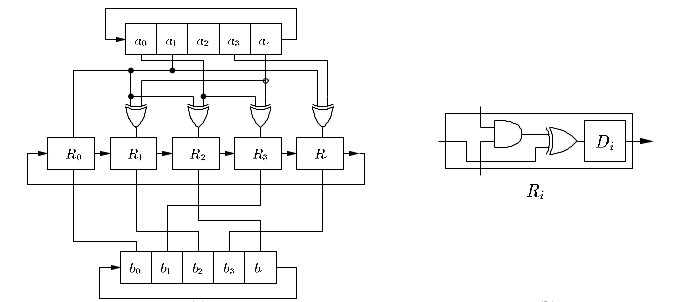
\includegraphics[scale=0.3]{./SMPO.png}}
    \caption{5-bit SMPO}
  \label{fig:SMPO}
  \end{figure}

Similarly, build elimination ideal for all gates/operations and induce
initial states of latches. However, instead of eliminating all variables
to one, this example adopts abstraction term order from \ref{thm:abs}
and keeps the polynomial contains function between output and inputs.
Here the lex ordering is $\{others\} > R > \{A, B\}$, and objective
polynimial is $R + \F(A, B)$. \par

Apply this approach to calculate image in BFS traversal, but modify 
\ref{alg:BFS} to make it adapt 6 steps reachable states enumeration.
The result is $R + AB$, which validates the function of this circuit.

\end{Example}

%%%%%%%%%%%%%%%%%%%% The bibliography %%%%%%%%%%%%%%%%%%%%%%%%%%%%
\bibliographystyle{ieee}
\bibliography{oldlogic,logic}

\end{document}

%%%%%%%%%%%%%%%%%%%%%%%%%%%  End of IEEEsample.tex  %%%%%%%%%%%%%%%%%%%%%%%%%%%
